%%
%% Author: Dario Chinelli
%% begin 2019-12-04
%% last mod 2022-02-02
%%

% Preamble
\documentclass[class=article, crop=false]{standalone}

% Packages
\usepackage{tikz}
\usetikzlibrary{positioning}

% Document
\begin{document}


\begin{figure}[ht]
\begin{minipage}[c]{0.5\linewidth}
\centering
\resizebox{0.5\textwidth}{!}{%
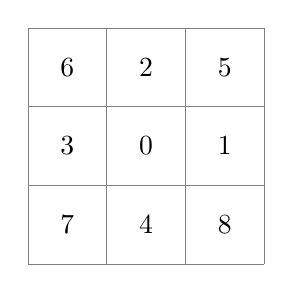
\begin{tikzpicture}
% Lines
\draw[step=1cm, gray, very thin] (0,0) grid (3,3);
% Nodes
\draw (1.5,1.5) node[black] {0};
\draw (2.5,1.5) node[black] {1};
\draw (1.5,2.5) node[black] {2};
\draw (0.5,1.5) node[black] {3};
\draw (1.5,0.5) node[black] {4};
\draw (2.5,2.5) node[black] {5};
\draw (0.5,2.5) node[black] {6};
\draw (0.5,0.5) node[black] {7};
\draw (2.5,0.5) node[black] {8};
\end{tikzpicture}
}%
\captionsetup{width=.8\linewidth}
\caption{This figure shows the indexes associated to each possible transitions from the center to the another cells. To every transition is associated a number: the index $k$.}
\label{fig:D2Q9_k}
\end{minipage}
\begin{minipage}[c]{0.5\linewidth}
\centering
\resizebox{0.5\textwidth}{!}{%
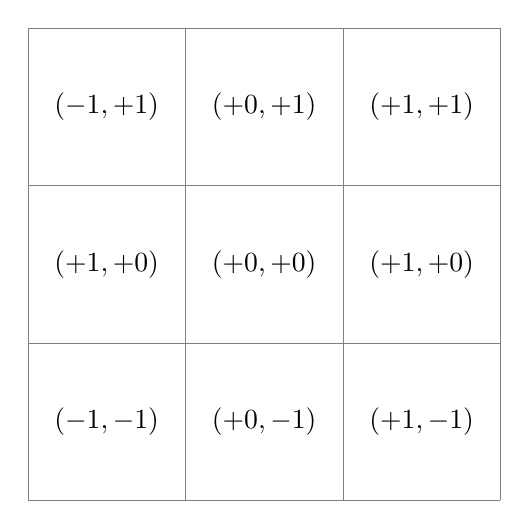
\begin{tikzpicture}
% Lines
\draw[step=2cm, gray, very thin] (0,0) grid (6,6);
% Nodes
\draw (3,3) node[black] {$(+0,+0)$};
\draw (5,3) node[black] {$(+1,+0)$};
\draw (3,5) node[black] {$(+0,+1)$};
\draw (1,3) node[black] {$(+1,+0)$};
\draw (3,1) node[black] {$(+0,-1)$};
\draw (5,5) node[black] {$(+1,+1)$};
\draw (1,5) node[black] {$(-1,+1)$};
\draw (1,1) node[black] {$(-1,-1)$};
\draw (5,1) node[black] {$(+1,-1)$};
\end{tikzpicture}
}%
\captionsetup{width=.9\linewidth}
\caption{Given the initial position at the center square, this is a representation of the change in coordinates to the next cell. The notation represents the variation along $x$ and $y$ axes, as $\Delta x, \Delta y$, from the initial position $(x_0, y_0)$.}
\label{fig:D2Q9_c}
\end{minipage}
\end{figure}


\end{document}
